
\section{Introducci�n}
\begin{frame}{Reconocimiento de Actividades Humanas}

\framesubtitle{Definici�n del Problema}
\begin{overprint}
\onslide<1> 
\begin{quote}
Determinar las acciones o comportamientos de uno o m�s individuos
a partir de datos ambiguos capturados por sensores situados en el
entorno. 
\begin{flushright}
{\small{}\emph{{\small{}{[}Bao and Intille, 2004, Chen et al., 2012, Reyes Ortiz,
2015{]}}}}
\par\end{flushright}{\small \par}
\end{quote}
\onslide<2> 
\begin{block}<2>{Nota}
\emph{}El problema es conocido por sus siglas \structure{HAR} en
ingl�s \emph{(Human Activity Recognition})
\end{block}
\end{overprint}
\begin{center}
\begin{minipage}[t]{0.7\columnwidth}%
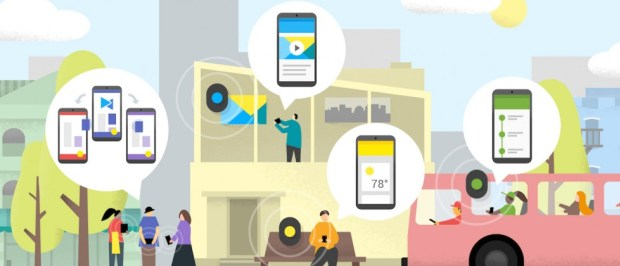
\includegraphics[width=1\textwidth]{intro/graphics/sensor-environment}

\begin{spacing}{0}
\noindent \textcolor{darkgray}{\emph{\tiny{}\copyright Beacons, Google
Developers}}{\tiny \par}
\end{spacing}
%
\end{minipage}
\par\end{center}

\end{frame}
%
\begin{frame}{�Que es HAR?}

\setbeamercovered{transparent}

\framesubtitle{Definici�n del Problema}
\begin{itemize}[<+->]
\item Es un t�pico de investigaci�n multidisciplinario que busca dise�ar
algoritmos para:
\begin{itemize}
\item Capturar movimientos de individuos en interacci�n con su entorno 
\item Realizar aprendizaje e inferencia
\item Proveer informaci�n de contexto 
\end{itemize}
\end{itemize}
\begin{overprint}
\onslide<2> 
\begin{center}
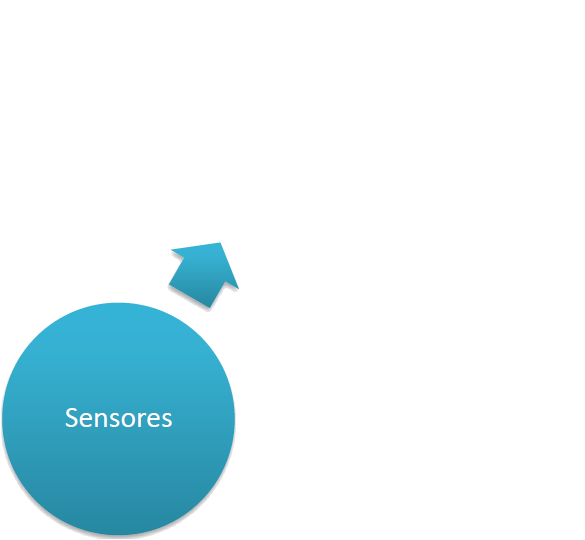
\includegraphics[width=4.5cm]{intro/graphics/areas-1}
\par\end{center}
\onslide<3> 
\begin{center}
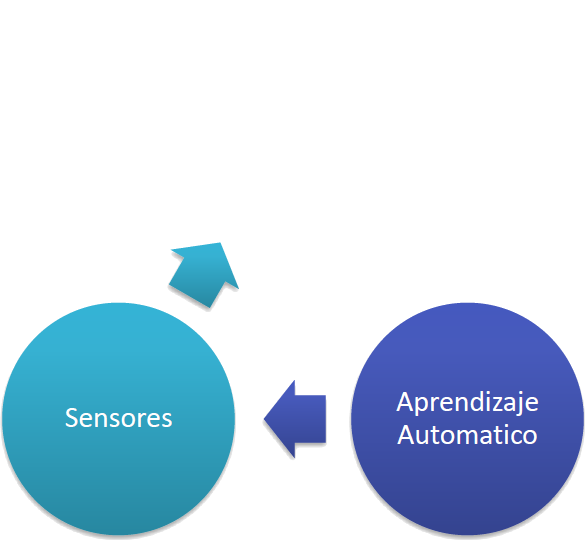
\includegraphics[width=4.5cm]{intro/graphics/areas-2}
\par\end{center}
\onslide<4> 
\begin{center}
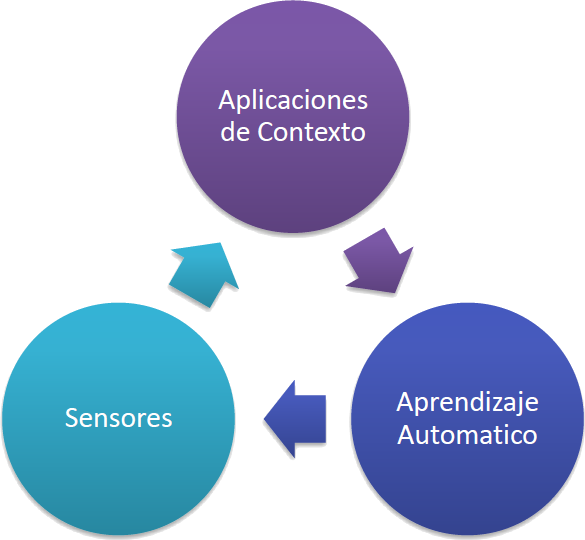
\includegraphics[width=4.5cm]{intro/graphics/areas-3}
\par\end{center}

\end{overprint}
\end{frame}
%
\begin{frame}{Motivaci�n}

\framesubtitle{Definici�n del Problema}

\setbeamercovered{transparent}\setlength\columnsep{0pt}
\begin{columns}

\column{0.5\textwidth}
\begin{itemize}
\item El \structure{contexto} es primordial para los sistemas inteligentes 
\end{itemize}
\begin{spacing}{0.5}

\pause{}
\end{spacing}
\begin{itemize}
\item Avances en tecnolog�as de \structure{computaci�n m�vil} y \structure{sensores} 
\end{itemize}
\begin{spacing}{0.5}

\pause{}
\end{spacing}
\begin{itemize}
\item Uso intensivo de \structure{tel�fonos m�viles modernos} en la vida
diaria.
\end{itemize}
\begin{spacing}{0.5}

\pause{}
\end{spacing}
\begin{itemize}
\item Popularidad de \structure{aplicaciones m�viles} de contexto en 
\begin{itemize}
\item el cuidado personal, 
\item la movilidad y 
\item la asistencia en la vida diaria 
\end{itemize}
\end{itemize}

\column{0.5\textwidth}
\begin{overprint}
\onslide<1> 


\includegraphics[width=1\textwidth]{intro/graphics/context1}

\begin{spacing}{0}
\noindent \emph{\tiny{}\copyright Connected Social Media, Intel}{\tiny \par}
\end{spacing}
\onslide<2> 

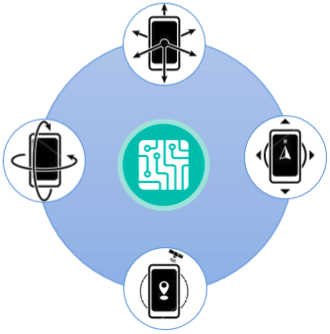
\includegraphics[width=1\textwidth]{intro/graphics/sensors}
\onslide<3> 

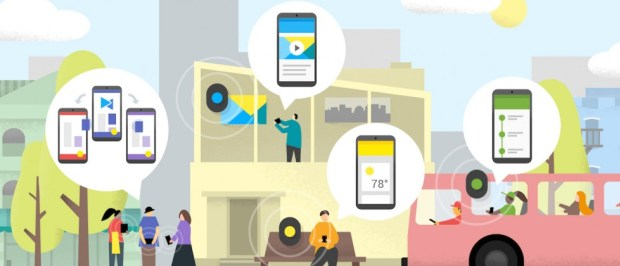
\includegraphics[bb=100bp 0bp 520bp 266bp,clip,width=1\textwidth]{intro/graphics/sensor-environment}

\begin{spacing}{0}
\noindent \emph{\tiny{}\copyright Beacons, Google Developers}{\tiny \par}
\end{spacing}
\onslide<4-> 

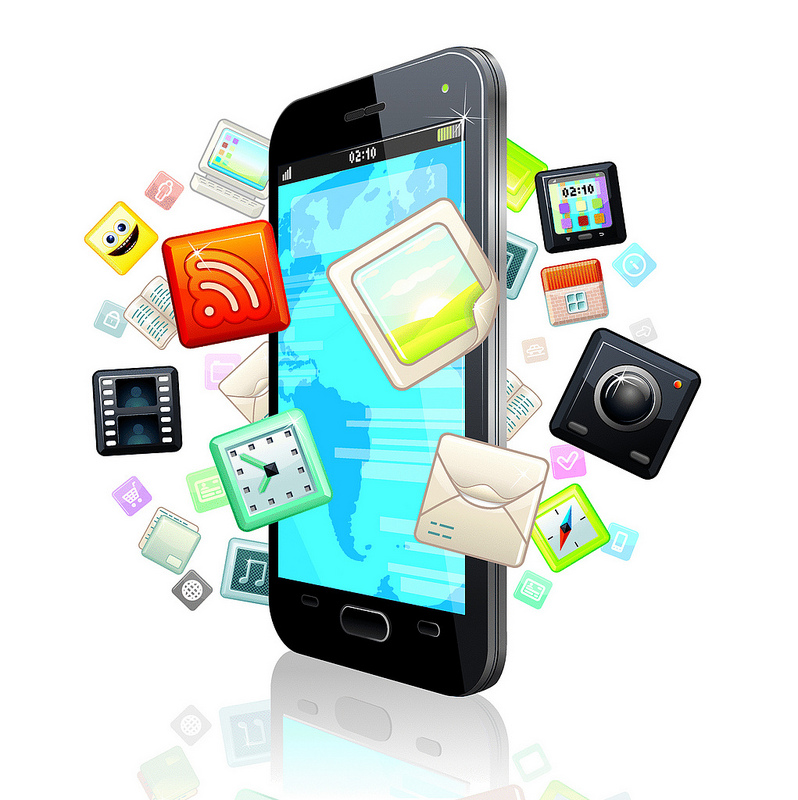
\includegraphics[width=1\textwidth]{intro/graphics/mobile-phone}

\begin{spacing}{0}
\noindent \emph{\tiny{}\cc Mobile Dev, Pinterest}{\tiny \par}
\end{spacing}
\end{overprint}
\end{columns}

\end{frame}
%
\begin{frame}{Contexto}

\framesubtitle{Definici�n del Problema}

Medio de interacci�n que representa el estado de la informaci�n f�sica,
emocional, social, entre otros. \emph{{[}Dey and Abowd, 2000{]}}
\begin{uncoverenv}<2>
\begin{columns}[t]

\column{0.5\textwidth}
\begin{itemize}
\item Ubicaci�n 
\item Identidad 
\item Actividad f�sica
\item Tiempo
\item Social
\end{itemize}

\column{0.5\textwidth}
\begin{center}
\textcolor{darkgray}{\emph{\tiny{}}}%
\noindent\begin{minipage}[t]{1\columnwidth}%
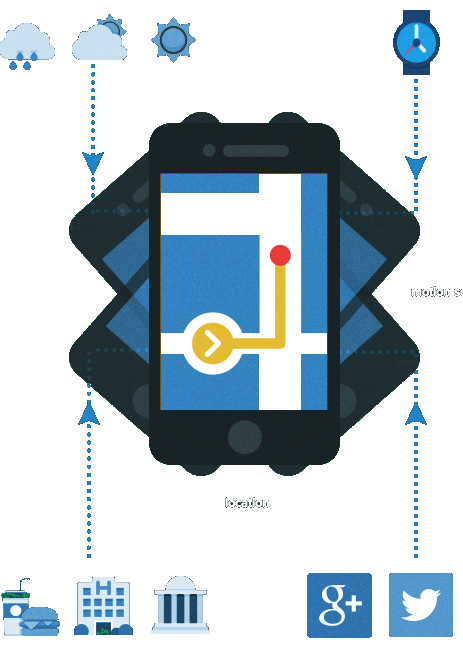
\includegraphics[width=0.65\textwidth]{intro/graphics/context2}\textcolor{darkgray}{\emph{\tiny{}\copyright
Toptal.io}}%
\end{minipage}
\par\end{center}{\tiny \par}

\end{columns}

\end{uncoverenv}

\end{frame}
%
\begin{frame}{HAR en Android}

\framesubtitle{Definici�n del Problema}

En la actualidad \emph{\textbf{\emph{Google Play Services}}} es la
�nica librer�a \structure{HAR} de uso libre para aplicaciones m�viles
de terceros.
\begin{overprint}
\onslide<1> 

\begin{figure}
\caption{Arquitectura de \protect\structure{HAR} en \protect\emph{Android}}

\centering{}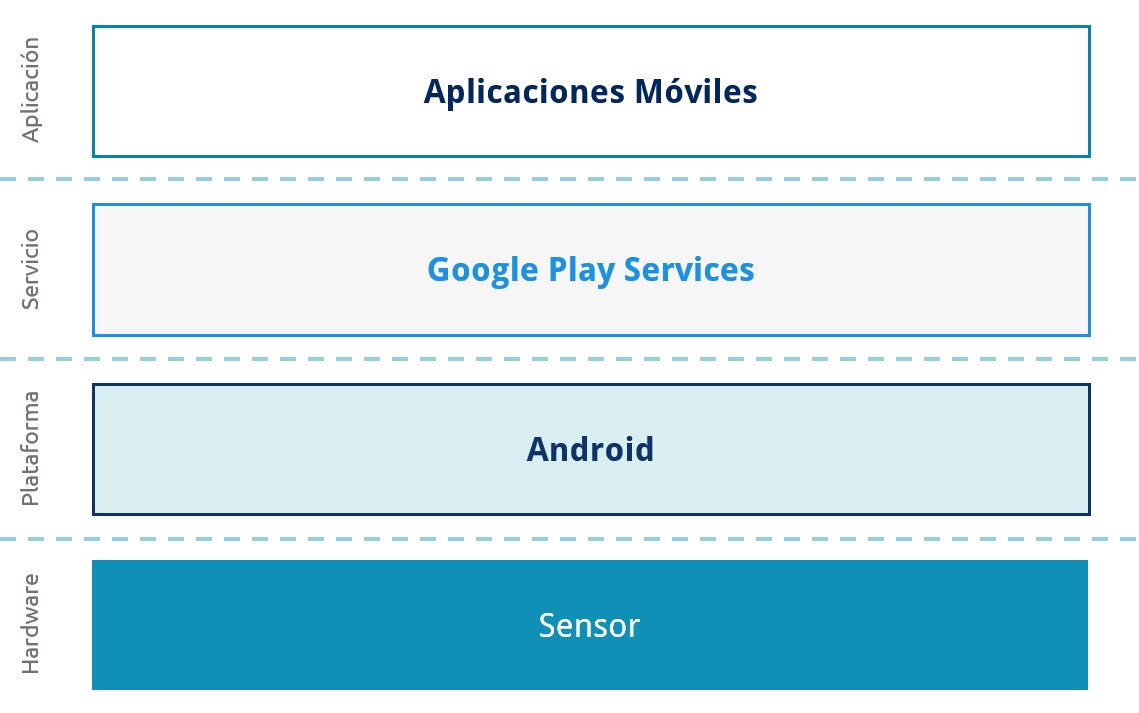
\includegraphics[width=0.65\textwidth]{intro/graphics/har_stack}
\end{figure}

\onslide<2> 
\begin{itemize}
\item No es de c�digo abierto (\structure{open source}).
\item Es de libre utilizaci�n pero no puede ser mejorado y extendido de
forma \structure{colaborativa}.
\item No existe una herramienta de software libre para fines pr�cticos e
investigaci�n equivalente con respecto a \structure{HAR}.
\end{itemize}
\end{overprint}
\end{frame}

